\documentclass{article}
\usepackage{graphicx}
%\usepackage[utf8]{inputenc}
\usepackage{geometry}
\usepackage{amsmath}

\begin{document}

\title{Lift event-based control - report}
\author{Cezary Dynak, Marek Frydrysiak, Dominik Koszuk, Michal Oleszczyk} 
\date{\today}
\maketitle

\section{High-level description}

Goal of this project is to create simulator an controller for multi lift
system. It will be parametrized by the number of lifts and the number
of floors. On each floor there are two buttons (let's call them eXternal),
to call any lift for going up or down. Inside lifts there are as many buttons,
as the number of floors, for choosing desired floor from inside. Controller
should optimize lifts movements.

\section{Automaton description}

\begin{figure}
  \centering
  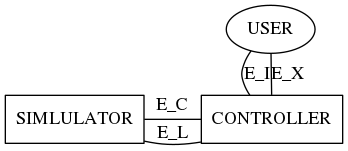
\includegraphics{img/simulator_controller.png}
  \caption{DES graph}
\end{figure}

\[
G = (E, S, f, \Gamma, s_0, S_M)
\]

%\newpage
% jeden
\subsection{States}

\[
S = [W, P, Q]
\]

\subsubsection{Lift states}

\[ W=[w_1, w_2, ..., w_i, ..., w_l ]\]
where:
\begin{itemize}
  \item \(l\) - number of lifts
\end{itemize}

\[ w_i = [d_i, o_i, f_i, m_i] \]
where:

\(d \in \{0,1\}\)
\begin{itemize}
  \item \(0\) - down
  \item \(1\) - up
\end{itemize}

\(o \in \{0,1\}\)
\begin{itemize}
  \item \(0\) - closed
  \item \(1\) - open
\end{itemize}

\(f \in \{0,1,...,i,...,n\}\)
\begin{itemize}
  \item \(i\) - last reached floor
  \item \(n\) - number of floors
\end{itemize}

\subsubsection{Internal buttons states}

\[ P = [p_1, p_2, ..., p_i, ..., p_n] \]
where:
\begin{itemize}
  \item \(n\) - number of floors
\end{itemize}

\[ p_i = [g_{u_i}, g_{d_i}] \]
where:
\(g_{u_i} \in \{0,1\}\)
\begin{itemize}
  \item 0 - not pushed
  \item 1 - pushed
\end{itemize}
\(g_{d_i} \in \{0,1\}\)
\begin{itemize}
  \item 0 - not pushed
  \item 1 - pushed
\end{itemize}


\subsubsection{External buttons states}
\[ Q = [q_1, q_2, ..., q_i, ..., q_l] \]
where:
\begin{itemize}
  \item \(l\) - number of lifts
\end{itemize}
\[q_i = [b_0, b_1, ..., b_i, ..., b_n] \]
\(b_i \in \{0,1\} \)
\begin{itemize}
  \item 0 - not pushed
  \item 1 - pushed
\end{itemize}



%\newpage
% dwa
\subsection{Events}

\[
E = E^l \cup E^c \cup E^x \cup E^i
\]

\[
E^i = [\text{lift\_nr},\text{button\_nr}]
\]

\(\text{direction} \in \{0,1\}\)

\[
E^x = [\text{lift\_nr}, \text{command}]
\]

\(\text{command} \in \{0,1,2,3,4\}\)

\[
E^c = [\text{lift\_nr}, \text{ACK}]
\]

\(\text{ACK} \in \{0,1,2,3\}\)

%\newpage
% trzy
\subsection{Transitions}

\section{Example}

Parameters:
\begin{itemize}
  \item number of lifts: 2,
  \item number of floors: 3.
\end{itemize}

\[
S = [ [d_1, o_1, f_1, m_1], [d_2, o_2, f_2, m_2] ]
\]
\[
P = [ [g_{u_0}, g_{d_0}], [g_{u_1}, g_{d_1}], [g_{u_2}, g_{d_2}] ]
\]
\[
Q = [ [b_{1_0},b_{1_1},b_{1_2}], [b_{2_0},b_{2_1},b_{2_2}] ]
\]
\[
W=[S,P,Q]
\]

\end{document}
